\documentclass{article}
\usepackage[utf8]{inputenc}

\usepackage{fullpage}
\usepackage{amsmath}
\usepackage{amsthm}
\usepackage{amsfonts}
\usepackage{amssymb}
\usepackage{enumerate}
\usepackage{color}

\usepackage{float}
\usepackage{graphicx}

\usepackage{hyperref}
\usepackage{cleveref}

\usepackage{todonotes}
\usepackage{listings}
\usepackage{tikz}
\usetikzlibrary{bayesnet}

\newcommand{\dd}{\mathrm{d}}

\newtheorem{theorem}{Theorem}
\newtheorem{lemma}[theorem]{Lemma}

\theoremstyle{definition}
\newtheorem{definition}{Definition}
\newtheorem{example}{Example}


\title{An Algebra on Tail Behaviour for Informing Inference Algorithm Design}

\begin{document}

\maketitle

\section{Introduction}
Our objective is to construct an algebra on the tail behaviour of one-dimensional distributions. For multi-dimensional distributions, we are primarily focused on tail behaviour of the marginals. The algebra will include exponential, Gaussian, log-normals, and power law tails, and form a commutative semiring under addition and multiplication (no inverses), while supporting powers, and some exponential and logarithmic operations. The complexities of the exact algebra for random variables (e.g. convolution) necessitate some approximations that will be suitable for most purposes. 

\subsection{Riemannian-Manifold MCMC}
\label{ssec:mcmc}

Among the most commonly used MCMC algorithms is the Metropolis-adjusted Langevin algorithm (MALA), based on discretizations of Langevin diffusion:
\[
\dd X_t = -\tfrac12 \nabla \log(X_t) \dd t + \dd B_t,
\]
where $B_t$ is Brownian motion. 

\begin{theorem}\label{thm:nmc-ergodic}
    From \cite{roberts1996exponential} theorem 4.3, MALA is not geometrically ergodic
    in the presence of heavy-tails ($\nabla  \log \pi(x) \to 0$).
    However, theorem 2.3 implies the Newtonian Monte-Carlo algorithm's use of the Hessian to define a metric tensor ensures the continuous
    time Langevin diffusion is exponentially ergodic. 
\end{theorem}
Our algebra may be used
to statically analyze a PPL program (representing a probabilistic model) and
recommend usage of potentially more expensive Riemannian methods.

\subsection{Proposal distributions}

Proposal distributions $q(x)$ are utilized in importance sampling, Metropolis-Hastings,
and variational inference, where the importance ratio $w(x) = \frac{p(x)}{q(x)}$ plays a
central role in their analysis. In particular, after establishing bounded variance of $w$ one
can apply Cauchy-Schwarz to yield efficient estimation procedures. For bounded variance, notice
\begin{align*}
    \text{Var}_q w
    &= \int_x \frac{p^2(x)}{q(x)} dx - 1
\end{align*}
Restricting comparison to polynomial orders, for $\int_1^\infty \frac{p^2(x)}{q(x)} dx$
to converge we must have $\frac{p^2(x)}{q(x)} = O(x^{-(1+\epsilon)})$ (with
upper bound $\frac{1+\epsilon}{\epsilon}$).

\begin{theorem}\label{thm:bdd-importance-ratio}
    If $p \in \mathcal{L}_\beta^2$ then $q \in \mathcal{L}_\alpha^2$ for $\alpha < 2 \beta$.
\end{theorem}

% Prior work (\cite{jaini2020tails}, TODO: cite NeurIPS submission) investigated
% the use of heavy-tailed variational families for variational inference, where
% tail parameters are jointly optimized as part of training.

Our algebra provides upper bounds on tail-coefficients which can be used as initializations
for the variational approximations. In doing so, we guarantee that proposal distributions $q(x)$ are at least as heavy as targets $p(x)$.

\section{Classes of Tail Behaviour}

\begin{definition}
The set of \emph{exponential-type densities} with scale $\alpha$ and exponent $\rho$, denoted $\mathcal{E}_\alpha^\rho$ is comprised of random variables $X$ satisfying
\[
\mathbb{P}(|X| \geq x) = \mathcal{O}(e^{-\alpha x^\rho}).
\]
Similarly, the set of \emph{logarithmic-type densities} with scale $\alpha$ and exponent $\rho$, denoted $\mathcal{L}_\alpha^\rho$, is comprised of random variables $X$ satisfying
\[
\mathbb{P}(|X| \geq x) = \mathcal{O}(e^{-\alpha (\log x)^\rho}).
\]
For brevity, we let $\mathcal{E}^\rho = \bigcup_{\alpha > 0} \mathcal{E}_\alpha^\rho$, $\mathcal{L}^\rho = \bigcup_{\alpha > 0} \mathcal{L}_\alpha^\rho$,  $\mathcal{E}=\bigcup_{\rho>0} \mathcal{E}^\rho$ and $\mathcal{L}=\bigcup_{\rho>0} \mathcal{L}^\rho$. We let $\mathcal{P} = \mathcal{E} \cup \mathcal{L}$ denote the set of viable random variables under this framework. 
\end{definition}

The tail behaviour is encoded by three properties: whether $X \in \mathcal{E}$ or $X \in \mathcal{L}$; the scale $\alpha$; and the exponent $\rho$. The collection of admissible random variables encompasses the following four classes:
\begin{enumerate}[(I)]
\item \textbf{Exponential:} $X \in \mathcal{E}_\alpha^1$ implies $\mathbb{P}(|X| \geq x) = \mathcal{O}(e^{-\alpha x})$
\item \textbf{Gaussian:}  $X\in\mathcal{E}_{\alpha}^{2}$ implies $\mathbb{P}(X\geq x)=\mathcal{O}(e^{-\alpha x^{2}})$.
\item \textbf{Power laws:} $X\in\mathcal{L}_{\alpha}^{1}$, implies $\mathbb{P}(X\geq x)=\mathcal{O}(x^{-\alpha})$.
\item \textbf{Log-normal:} $X\in\mathcal{L}_{\alpha}^{2}$, implies $\mathbb{P}(X\geq x)=\mathcal{O}(e^{-\alpha(\log x)^{2}})$.
\end{enumerate}

\section{Operations}

\paragraph{Ordering.}
First, we can assign a total ordering to random variables in the sets $\mathcal{E}$ and $\mathcal{L}$ over the equivalence classes specified by the parameters $\alpha$ and $\rho$. This ordering is defined so that $X > Y$ if $X$ has heavier tails than $Y$. In tail behaviour, $X \equiv Y$ if $X,Y$ belong to the same class with equivalent scales $\alpha$ and exponents $\rho$. Furthermore, $X > Y$ if one of the following holds:
\begin{enumerate}[(i)]
\item $X \in \mathcal{L}, Y \in \mathcal{E}$.
\item Both $X,Y \in \mathcal{L}$, but $X \in \mathcal{L}^\rho, Y \in \mathcal{L}^\lambda$,  and $\rho < \lambda$.
\item Both $X,Y \in \mathcal{E}$, but $X \in \mathcal{E}^\rho, Y \in \mathcal{E}^\lambda$, and $\rho < \lambda$.
\item Both $X,Y \in \mathcal{L}^\rho$, but $X \in \mathcal{L}_\alpha^\rho, Y \in \mathcal{L}_\beta^\rho$, and $\alpha < \beta$.
\item Both $X,Y \in \mathcal{E}^\rho$, but $X \in \mathcal{E}_\alpha^\rho, Y \in \mathcal{E}_\beta^\rho$, and $\alpha < \beta$.
\end{enumerate}

\paragraph{Exponential and Logarithm.}
By design, $X \in \mathcal{L}_\alpha^\rho$ if and only if $\log X \in \mathcal{E}_\alpha^\rho$ --- this is easy to show by a change of variables. Similarly, if $Y \in \mathcal{E}_\alpha^\rho$, then $\exp Y \in \mathcal{L}_\alpha^\rho$. If $Y \in \mathcal{E}_\alpha^\rho$, then $\log Y$ is lighter than any exponential density, so we are free to take $\log Y \in \mathcal{E}_\alpha^{\tilde{\infty}}$, where $\tilde{\infty}$ is a suitably large number. On the other hand, if $X \in \mathcal{L}_\alpha^\rho$, then $\exp X$ is heavier than any power law, falling into the family of \emph{super-heavy tails}. Our analysis is not capable of treating these variables, so we leave $\exp X$ to be undefined. 

\paragraph{Powers.} If $X \in \mathcal{E}_\alpha^\rho$ (resp. $\mathcal{L}_\alpha^\rho$) then $X^\beta \in \mathcal{E}_\alpha^{\rho / \beta}$ (resp. $\mathcal{L}_\alpha^{\rho / \beta}$). If $\beta < 0$, then $X^{\beta} = (X^{-1})^{|\beta|}$, which will be covered by the reciprocal case later.

\paragraph{Multiplication by a Constant.}
It can be readily seen from the definitions that if $X \in \mathcal{E}_\alpha^\rho$, then for any $c \in \mathbb{R}$, $c X \in \mathcal{E}_{\alpha / |c|^\rho}^\rho$. On the other hand, the tails of logarithmic-type distributions are unaffected by constant factors, so if $X \in \mathcal{L}_\alpha^\rho$, then $c X \in \mathcal{L}_\alpha^\rho$. 


\paragraph{Reciprocal.}
Unfortunately, determining the tail behaviour of the reciprocal $X^{-1}$ from the tail behaviour of $X$ is technically ill-posed, as it depends on the probability density of $X$ about zero. For example, a $t_\nu$-distributed random variable is defined as a ratio $\sqrt{\nu} X / Y$ where $X,Y \in \mathcal{E}_{1/2}^2$. This is true for any $\nu > 1$. Therefore, no rule depending only on the scale and exponent is capable of predicting the degrees of freedom $\nu$ in this setting. 
However, since the majority of heavy tails seem to arise in ratio distributions, it is critical to treat reciprocal operations. 
Fortunately, most cases will be covered by the following general rule shown in Lemma \ref{lem:Reciprocal}. 

\begin{lemma}
\label{lem:Reciprocal}
Suppose that $X$ is a random variable with bounded density $p_X$. Then $X^{-1} \in \mathcal{L}_1^1$. 
\end{lemma}
\begin{proof}
By a change of variables, the density of $X^{-1}$ is
\[
p_{X^{-1}}(x) = x^{-2}p_X(x^{-1}).
\]
Since $p_X$ is bounded, $p_{X^{-1}}(x) = \mathcal{O}(x^{-2})$ as $x \to \infty$, which implies the result.
\end{proof}

\paragraph{Addition.}
Addition is the first operation not covered by a simple change of variables. Of course, at complete generality, one can use the naive bound
\[
X + Y \equiv \max\{2 X, 2 Y\}.
\]
This turns out to be effective in most cases when the scales do not matter. The single exception occurs when $X,Y \in \mathcal{E}^\rho$ for $\rho \geq 1 $, in which case, the scale does matter. This case is covered by the following lemma, which assumes independence.
\begin{lemma}
\label{lem:sum}
Suppose that $X, Y \in \mathcal{E}^\rho$ are independent random variables for $\rho \geq 1$. If $X \in \mathcal{E}_\alpha^\rho$ and $Y \in \mathcal{E}_\beta^\rho$, then $X + Y \in \mathcal{E}_\sigma^\rho$ where
\[
\sigma = \begin{cases}
\min\{\alpha,\beta\}&\mbox{ if } \rho = 1 \\
(\alpha^{-\frac{1}{\rho-1}}+\beta^{-\frac{1}{\rho-1}})^{1-\rho} &\mbox{ if } \rho > 1.
\end{cases}
\]
\end{lemma}
\begin{proof}
We focus on the $\rho > 1$ case, since the $\rho = 1$ case follows by taking $\rho \to 1^+$. It also suffices to consider the case where $\limsup_{x \to \infty} \mathbb{P}(|X| > x^{1/\rho}) = -\alpha$ and $\limsup_{x\to\infty} \mathbb{P}(|Y| > x^{1/\rho}) = -\beta$, as the tail behaviour will be bounded above by this case. By Kasahara's Tauberian Theorem, 
\begin{align*}
\limsup_{\lambda \to \infty} \lambda^{-\frac{\rho}{\rho-1}}\log \mathbb{E}e^{\lambda |X|} &= \frac{\rho - 1}{\rho} (\alpha \rho)^{-\frac{1}{\rho-1}} \\
\limsup_{\lambda \to \infty} \lambda^{-\frac{\rho}{\rho-1}}\log \mathbb{E}e^{\lambda |Y|} &= \frac{\rho - 1}{\rho} (\beta \rho)^{-\frac{1}{\rho-1}},
\end{align*}
and since $X$ and $Y$ are independent,
\[
\limsup_{\lambda \to \infty} \lambda^{-\frac{\rho}{\rho-1}}\log \mathbb{E}e^{\lambda (|X|+|Y|)} = \frac{\rho - 1}{\rho} (\sigma \rho)^{-\frac{1}{\rho-1}},
\]
which, by the same theorem, implies that $\mathbb{P}(|X|+|Y|>x) = \mathcal{O}(e^{-\sigma x^\rho})$.
Since $|X+Y| \leq |X| + |Y|$, the result follows.
\end{proof}

\paragraph{Multiplication by a Random Variable.}
The next binary operation of interest is \emph{multiplication}. Using Cauchy's inequality, we can adopt the naive
\[
X \cdot Y \equiv \max\{X^2, Y^2\}.
\]
In the case where $X,Y \in \mathcal{E}$, this turns out to be reasonable. However, for any other use case, Breiman's lemma suggests that $X \cdot Y \equiv \max\{X, Y\}$. \todo{Perform Tauberian analysis to determine sharpness of these operations}.


\paragraph{Product of Densities.}

To handle the application of priors, it is necessary to support a product of densities operation acting on two random variables $X,Y$, denoted $X \& Y$, by
\[
p_{X \& Y}(x) = \frac{1}{\mathcal{Z}} p_X(x) p_Y(x),
\]
where $\mathcal{Z}$ is an appropriate normalizing constant and $p_X,p_Y,p_{X\& Y}$ are the densities of $X$, $Y$, and $X \& Y$, respectively.
Like addition of random variables, a simple naive bound
\[
X \& Y \equiv \min\{X, Y\},
\]
often suffices when $X,Y$ have different forms of their tails. If $X,Y \in \mathcal{E}^\rho$, $X \in \mathcal{E}_\alpha^\rho$, $Y \in \mathcal{E}_\beta^\rho$, then $X\& Y \in \mathcal{E}_{\alpha+\beta}^\rho$. Similarly, if $\rho > 1$, $X,Y \in \mathcal{L}^\rho$, $X \in \mathcal{L}_\alpha^\rho$, $Y \in \mathcal{L}_\beta^\rho$, then $X\& Y \in \mathcal{L}_{\alpha+\beta}^\rho$. The final exception lies in the $\rho \leq 1$ case, where the densities necessarily exhibit different tail behaviour to their survival functions $\mathbb{P}(|X| > x)$. Using Pareto densities as a model, we say that if $X \in \mathcal{L}_\alpha^\rho$ and $Y \in \mathcal{L}_\beta^\rho$ for $\rho \leq 1$, then $X \& Y \in \mathcal{L}_{\alpha+\beta-1}^\rho$.



\paragraph{Lipschitz Functions.}

There are many multivariate functions that cannot be readily represented in terms of the operations covered thus far. For these, it is important to specify the tail behaviour of pushforward measures under Lipschitz-continuous functions. Fortunately, this is covered by \cite[Proposition 1.3]{ledoux2001concentration}.
\begin{lemma}
For any Lipschitz continuous function $f:\mathbb{R}^d \to \mathbb{R}$ satisfying $\|f(x)-f(y)\|\leq L\|x -y\|$ for $x,y \in \mathbb{R}^d$, there is
\[
f(X_1,\dots,X_d) \equiv L \max\{X_1,\dots,X_d\}.
\]
\end{lemma}
H\"{o}lder-continuous functions can be represented as a composition of a power operation and a Lipschitz-continuous function. 

\paragraph{Conditioning.}
A primary application of sampling techniques is for Bayesian inference. To cover this use case, it is necessary to prescribe a procedure to deal with \emph{conditional distributions}. For this, we introduce a very simple approach involving inverses. 

Suppose that a random variable $X$ is dependent on a parameter $\theta$ and a latent random element $Z$ through a function $f$ by
\[
X = f(\theta; Z).
\]
Assuming that $f$ is invertible with respect to $\theta$, with inverse $f^{-1}$, it follows that
\[
\theta = f^{-1}(X; Z).
\]
It follows from the Doob-Dynkin lemma that the distribution of $\theta$ conditioned on $X = x$ is precisely that of $f^{-1}(x;Z)$.

\begin{example}
As a simple example, if $X \sim \mathcal{N}(\mu,\sigma^2)$, then since $X = \mu + \sigma Z$ for $Z \sim \mathcal{N}(0,1)$, $\mu = X - \sigma Z$ and so
\[
\mu \vert X = x \sim \mathcal{N}(x, \sigma^2).
\]
\end{example}

\section{New Algebra}

Consider a tail algebra for random variables with tails of the generalized gamma form:
\[
f_X(x) \sim c x^\nu e^{-\sigma x^\rho}
\]
The tail of a random variable $X$ of this form can be represented as a triple $(\nu,\sigma,\rho)$. Additionally, we require
\[
    \nu \in \mathbb{R}, \sigma > 0, \rho \in \mathbb{R}
\]
while noting that $\sigma = 0$ corresponds to the theory of regularly varying distributions.


\todo{Compare against Lemma 1.3.4 of \cite{mikosch}}
Tails of this form are  closed under addition: denoting the addition of random variables (additive convolution) by $\oplus$,
\[
(\nu_{1},\sigma_{1},\rho_{1})\oplus(\nu_{2},\sigma_{2},\rho_{2})
=\begin{cases}
\max\{(\nu_{1},\sigma_{1},\rho_{1}),(\nu_{2},\sigma_{2},\rho_{2})\} & \text{ if }\rho_{1}\neq\rho_{2}\text{ or }\rho_{1},\rho_{2}<1\\
\left(\nu_{1}+\nu_{2}+1,\min\{\sigma_{1},\sigma_{2}\},1\right) & \text{ if }\rho_{1}=\rho_{2}=1\\
(\nu_{1}+\nu_{2}+1-\frac{\rho}{2},(\sigma_{1}^{-\frac{1}{\rho-1}}+\sigma_{2}^{-\frac{1}{\rho-1}})^{1-\rho},\rho) & \text{ if }\rho=\rho_{1}=\rho_{2}>1
\end{cases}
\]
\todo{Chi squared distribution has both $\nu,\rho > 0$}
\todo{Student-T tail is exactly recovered }
where $\max$ selects the heavier tail. Similarly, powers and scalar products satisfy
\[
(\nu,\sigma,\rho)^m = \bigg(\frac{\nu+1}{m} - 1, \sigma, \frac{\rho}{m}\bigg),
\]
and $c(\nu,\sigma,\rho) = (\nu,|c|^{-1} \sigma,\rho)$. 
Tails are also (almost) closed under multiplication: denoting the multiplication of random variables (multiplicative convolution) by $\otimes$,
\[
(\nu_{1},\sigma_{1},\rho_{1})\otimes(\nu_{2},\sigma_{2},\rho_{2})
=\begin{cases}
\left(\frac{1}{\mu}\left(\frac{\nu_{1}}{|\rho_{1}|}+\frac{\nu_{2}}{|\rho_{2}|}-\frac{3}{2}\right),\sigma,\frac{1}{\mu}\right) & \text{ if }\rho_{1},\rho_{2}<0\\
\left(\frac{1}{\mu}\left(\frac{\nu_{1}}{\rho_{1}}+\frac{\nu_{2}}{\rho_{2}}-\frac{1}{2}\right),\sigma,\frac{1}{\mu}\right) & \text{ if }\rho_{1},\rho_{2}>0\\
(\nu_{1},0,0) & \mbox{ if }\rho_{1}\leq0,\rho_{2}>0 \\
(\max\{\nu_1,\nu_2\},0,0) & \mbox{ if }\rho_{1}=0,\rho_{2}=0
\end{cases}
\]
where $\mu=\frac{1}{|\rho_{1}|}+\frac{1}{|\rho_{2}|}=\frac{|\rho_{1}|+|\rho_{2}|}{|\rho_{1}\rho_{2}|}$ and $\sigma=\sigma(\sigma_{1}|\rho_{1}|)^{\frac{1}{\mu\rho_{1}}}(\sigma_{2}|\rho_{2}|)^{\frac{1}{\mu\rho_{2}}}$. 

\subsection{Relation with regular variation}

Both our theory as well as the theory of regularly varying functions represent functions modulo
asymptotic behavior.
\begin{definition}
    A positive measurable function $f$ is \emph{regularly varying at infinity} with index $\alpha \in \mathbb{R}$ if
    \[
        \lim_{x \to \infty} \frac{f(tx)}{f(x)} = t^{\alpha}\qquad\forall t > 0
    \]
    If $\alpha = 0$, then $f$ is \emph{slowly varying}
\end{definition}
However, our theory is strictly finer in that it may interpolate between
the regularly varying theory and sub-exponential theory which offers finer control. In particular, the
generalized gamma density $e^{-\sigma x^\rho}$ is neglected by the regularly varying theory.

\begin{lemma}
    $F$ with density $f$ is a regularly varying distribution with
    index $\alpha$ iff $f \sim (\alpha, \cdot, \cdot)$
\end{lemma}

\subsection{Application: importance sampling ratio}

\cite{vehtari2015pareto} propose stabilizing importance weights using a Pareto approximation to the importance weights. Can we use our algebra to avoid the empirical estimation procedure \cite{zhang2009new} into a symbolic analysis one?

Given probability densities $p$ and $q$ over a common support, we are interested in determining the tail index of
\[
    \frac{p(X)}{q(x)},\qquad X \sim q
\]
The elementary case is when we are interested in sampling $X \sim p$ over $\mathcal{X}$ and while $p$ may be intractable a readily sample-able proposal $q$ is available. 
So long as $p \ll q$, we need not worry about division by zero.
Note $p(X)$ and $q(X)$ are $\mathbb{R}_+$-valued random variables with high correlation if $q$ is chosen well. 

\textbf{Problem}: Heavy-tailed PDFs are usually not Lipschitz!

Even without heavy tails, consider $p = Exp(1)$ and $q = Exp(\theta)$. Then
$Y = p(X) = e^{-X}$ is the exponential transform of $X$ and has density 
\[
    \lvert \frac{1}{Y} \rvert e^{-\theta \log Y}
    = Y^{-\theta - 1}
\]
because $Y \geq 0$. Similarly, the density of $Z = q(X) = \theta e^{-\theta X}$ is given by
\[
\lvert \frac{1}{Z \theta} \rvert e^{(\log Z - \log \theta )}
= (\theta Z)^{-1-1}
\]
Cast into our algebra, we have that $Y = (-\theta-1,0,0)$ and $Z = (-2,0,0)$
so the reciprocal
\[
    Z^{-1} = (0, 0, 0)
\]
(TODO: improper distribution? or computation error?)


\section{Static analysis of probabilistic programs}

To conveniently express stochastic processes and automatically perform inference,
researchers oftentimes employ probabilistic programming languages. For closed-world
probabilistic programs (i.e. representing static graphical models), static analysis
may be performed prior to inference in order to inform and improve
inference through methods such as automatically marginalizing \cite{murray2018automated} 
or exploiting conjugacy relations \cite{hoffman2018autoconj}. In this section, we describe
how our heavy-tailed algebra can similarly be leveraged during static analysis of a
probabilistic program in order to detect and bound the tail behavior of heavy-tailed
random variables. Combined with \cref{thm:nmc-ergodic} and \cref{{thm:bdd-importance-ratio},
this leads to more informed inference algorithms which achieve strong guarantees even in the presence of heavy tails.

Consider the following PP:
\begin{lstlisting}
    X1 ~ Normal(0, 1)
    X2 = 2*X1
    X3 ~ Normal(0, 2)
    Y = X2 + X3
    Z1 = exp Y
    Z2 ~ StudentT(3)
    W = Z1 * Z2
\end{lstlisting}

Note that the random variables present in the program is fixed; only the values are random.
As a result, it is possible to construct an equivalent non-plated graph representation for the program
(e.g. by transforming the AST, or alternatively by tracing program execution)

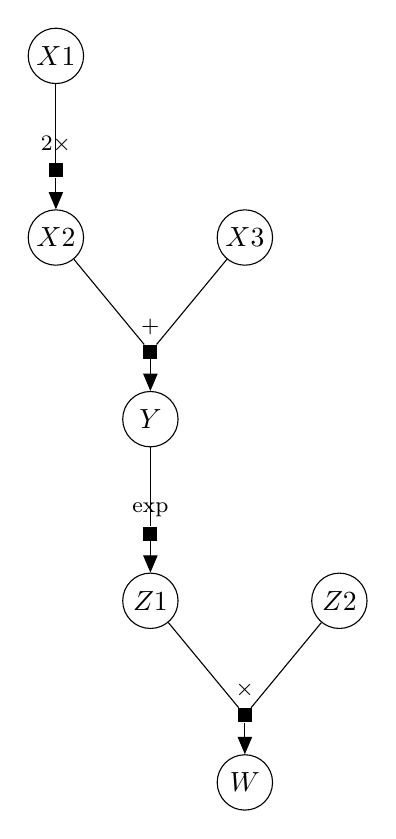
\begin{tikzpicture}
  \node[latent]                               (W) {$W$};
  \factor[above=of W] {mult-W} {$\times$} {} {};
  \node[latent, above=of mult-W, xshift=-1.2cm] (Z1) {$Z1$};
  \node[latent, above=of mult-W, xshift=1.2cm]  (Z2) {$Z2$};
  \factor[above=of Z1] {exp-Z1} {$\exp$} {} {};
  \node[latent, above=of exp-Z1] (Y) {$Y$};
  \factor[above=of Y] {plus-Y} {$+$} {} {};
  \node[latent, above=of plus-Y, xshift=-1.2cm] (X2) {$X2$};
  \node[latent, above=of plus-Y, xshift=1.2cm] (X3) {$X3$};
  \factor[above=of X2] {t2-X3} {$2\times$} {} {};
  \node[latent, above=of t2-X3] (X1) {$X1$};
  
  \factoredge {Z1, Z2} {mult-W} {W};
  \factoredge {Y} {exp-Z1} {Z1};
  \factoredge {X2, X3} {plus-Y} {Y};
  \factoredge {X1} {t2-X3} {X2};
\end{tikzpicture}

To statically analyze the program with our algebra, the first step is to annotate all ``primitive'' distributions
(i.e. nodes given by \texttt{sample} statements ``~'', no ancestors in the PGM) with their tail classes

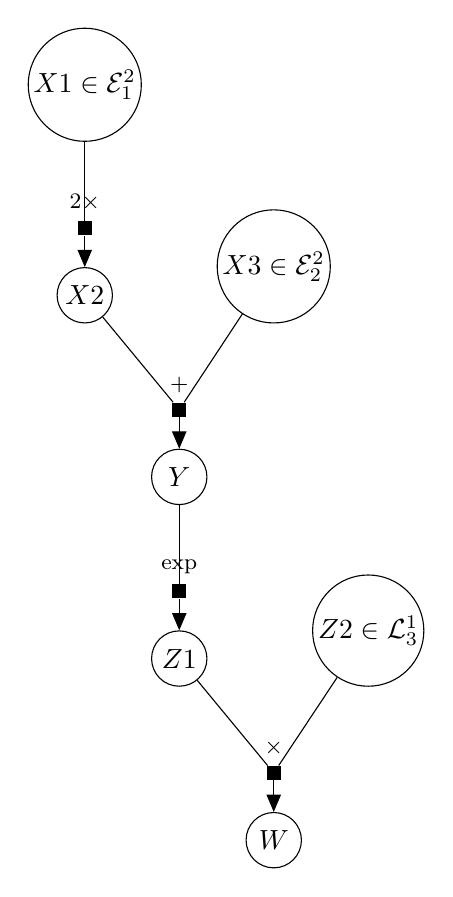
\begin{tikzpicture}
  \node[latent]                               (W) {$W$};
  \factor[above=of W] {mult-W} {$\times$} {} {};
  \node[latent, above=of mult-W, xshift=-1.2cm] (Z1) {$Z1$};
  \node[latent, above=of mult-W, xshift=1.2cm]  (Z2) {$Z2 \in \mathcal{L}^1_3$};
  \factor[above=of Z1] {exp-Z1} {$\exp$} {} {};
  \node[latent, above=of exp-Z1] (Y) {$Y$};
  \factor[above=of Y] {plus-Y} {$+$} {} {};
  \node[latent, above=of plus-Y, xshift=-1.2cm] (X2) {$X2$};
  \node[latent, above=of plus-Y, xshift=1.2cm] (X3) {$X3 \in \mathcal{E}^2_2$};
  \factor[above=of X2] {t2-X3} {$2\times$} {} {};
  \node[latent, above=of t2-X3] (X1) {$X1 \in \mathcal{E}^2_1$};
  
  % Connect the nodes
  \factoredge {Z1, Z2} {mult-W} {W};
  \factoredge {Y} {exp-Z1} {Z1};
  \factoredge {X2, X3} {plus-Y} {Y};
  \factoredge {X1} {t2-X3} {X2};
\end{tikzpicture}

Next, for each child node whose parents are completely annotated, a matching algebra rule
is applied to derive its tail class. If no matching rule exists, then our algebra is unable to
bound the rate of tail decay of that node and any of its ancestors. In this example,
``multiplication by a constant'' is applied for $X2$, ``addition'' for $Y$, ``exponential and logarithm'' for $Z1$,
and finally ``multiplication by a random variable'' for $W$.

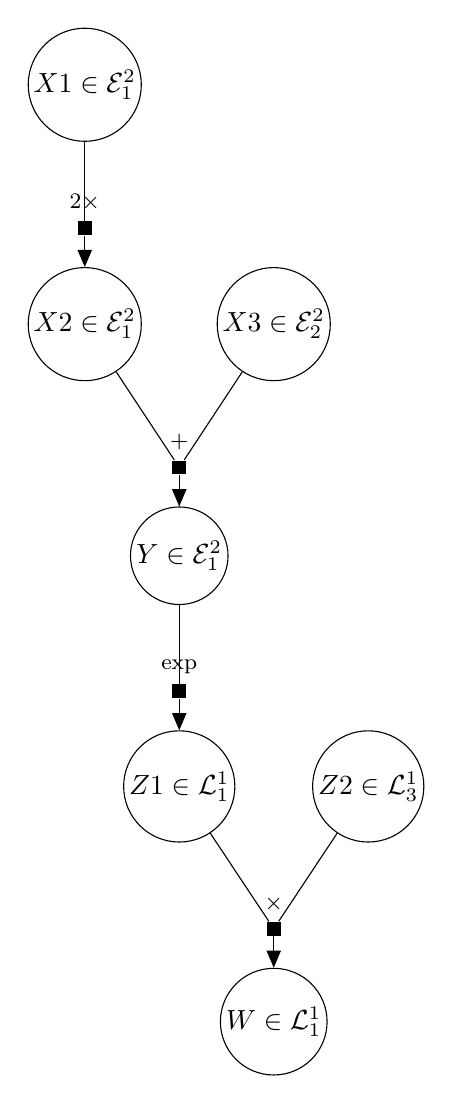
\begin{tikzpicture}
  \node[latent]                               (W) {$W \in \mathcal{L}^1_1$};
  \factor[above=of W] {mult-W} {$\times$} {} {};
  \node[latent, above=of mult-W, xshift=-1.2cm] (Z1) {$Z1 \in \mathcal{L}^1_1$};
  \node[latent, above=of mult-W, xshift=1.2cm]  (Z2) {$Z2 \in \mathcal{L}^1_3$};
  \factor[above=of Z1] {exp-Z1} {$\exp$} {} {};
  \node[latent, above=of exp-Z1] (Y) {$Y \in \mathcal{E}^2_1$};
  \factor[above=of Y] {plus-Y} {$+$} {} {};
  \node[latent, above=of plus-Y, xshift=-1.2cm] (X2) {$X2 \in \mathcal{E}^2_1$};
  \node[latent, above=of plus-Y, xshift=1.2cm] (X3) {$X3 \in \mathcal{E}^2_2$};
  \factor[above=of X2] {t2-X3} {$2\times$} {} {};
  \node[latent, above=of t2-X3] (X1) {$X1 \in \mathcal{E}^2_1$};
  
  % Connect the nodes
  \factoredge {Z1, Z2} {mult-W} {W};
  \factoredge {Y} {exp-Z1} {Z1};
  \factoredge {X2, X3} {plus-Y} {Y};
  \factoredge {X1} {t2-X3} {X2};
\end{tikzpicture}

\section{Experiments}

\subsection{TODO: new toy experiments}

\begin{itemize}
    \item Chi square from squared Normal
    \item Cauchy from ratio distribution
    \item Standardized residual is Student-t distributed
    \item Kestern's law and iterated add/mult with iid random variables (?)
\end{itemize}

\subsection{Informing MCMC algorithm selection in Neal's heavy funnel}

Neal's funnel is a bivariate probability density commonly used to benchmark MCMC inference algorithm's ability to explore posterior distributions. Here, we consider a variant with anisotropic heavy tails where
\[
    z \sim t_\nu(\text{loc}=0, \text{scale}=10),
    x \mid z \sim N(\text{loc}=0, \text{scale}=e^{z/2})
\]
See \Cref{fig:neals-funnel}

\begin{figure}[h]
    \centering
    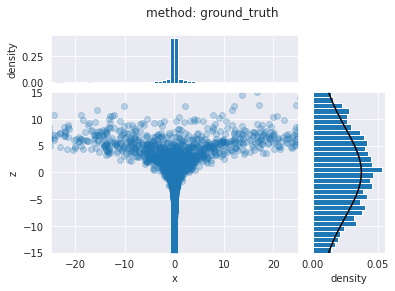
\includegraphics[width=0.3\textwidth]{figures/nf-1.png}
    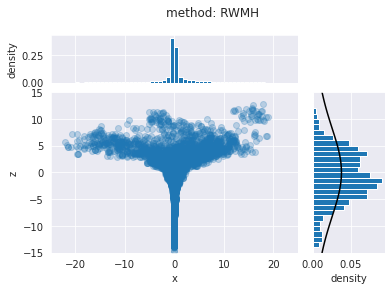
\includegraphics[width=0.3\linewidth]{figures/nf-2.png}
    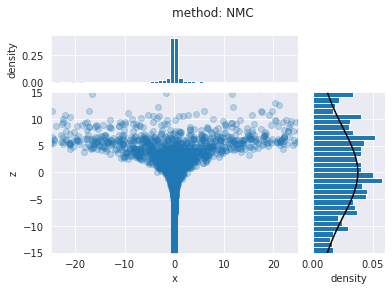
\includegraphics[width=0.3\linewidth]{figures/nf-3.png}
    \caption{Samples from Neal's heavy funnel (left), which both random walk Metropolis-Hastings (middle), NUTS (TODO) and Newtonian Monte Carlo (right) aim to approximate. The presence of a heavy-tailed $z$ necessitates a more sophisticated algorithm than MALA, and our algebra is able to detect this during static analysis to inform the selection of inference routine.}
    \label{fig:neals-funnel}
\end{figure}

\subsection{MCMC kernel selection for simulating an option price}

Let $X$ be the price of an underlying asset (e.g. a stock price). Paying $P$ to purchase a put option on $X$ with strike prise $S$ has payoff

$$V = 1(X \geq S) (X - S) - P$$

Consider MCMC simulations of this put option's value $V$. See \Cref{fig:option}.
Using the algebra, we may compute $V < X$ so by theory on importance sampling ratios
the proposal distribution for $V$ can be at least as heavy as $X$ while retaining bounded
variances. This suggests a ``informed heavy tailed proposer'' of $t_{\nu=\alpha(X)}$ which
exploits the result of our algebra to ensure bounded variances.

\begin{figure}[H]
    \centering
    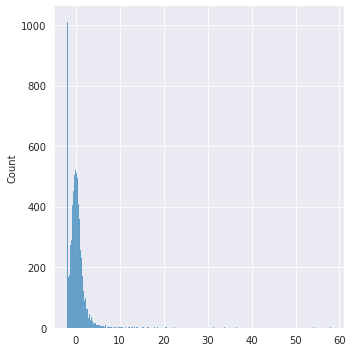
\includegraphics[width=0.3\textwidth]{figures/option-1.png}
    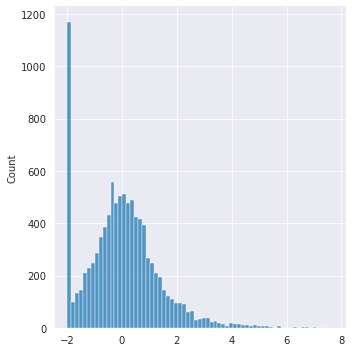
\includegraphics[width=0.3\textwidth]{figures/option-2.png}
    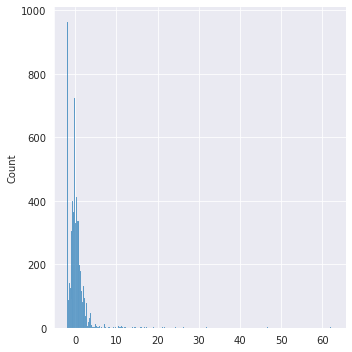
\includegraphics[width=0.3\textwidth]{figures/option-3.png}
    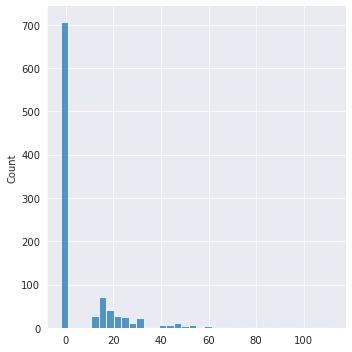
\includegraphics[width=0.3\textwidth]{figures/option-4.png}
    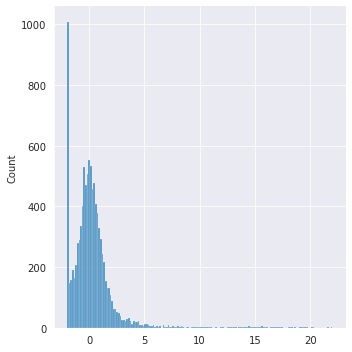
\includegraphics[width=0.3\textwidth]{figures/option-5.png}
    \caption{Empirical distributions of options prices from 
    (left to right, top to bottom) ground truth, RWMH, NMC, NUTS, and
    an informed heavy tailed proposer. The informed proposer has an accurate estimate of the
    $P(V=0)$ probability compared to RWMH and NUTS and generates samples comparable to the ground truth/NMC
    all without requiring computation of the Hessian like NMC.}
    \label{fig:option}
\end{figure}

\subsubsection{Additive time series}

Other applications may involve a time series with stochastic shocks at each time-step.
If these shocks are heavy-tailed, then repeated applications of \cref{lem:sum} allow
for controlling the tail behavior of forecasts.

\todo{MC (or VI?) for distribution of $x(T)$}

\begin{figure}[H]
    \centering
    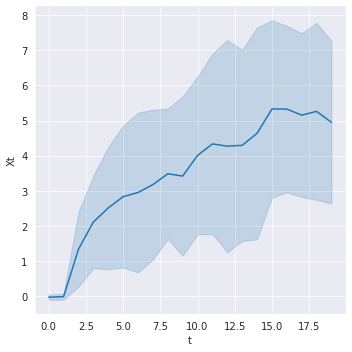
\includegraphics[width=0.4\textwidth]{figures/ar2.png}
    \caption{Empirical distribution of samples from an AR(2) heavy-tailed additive time series.
    The predictive distribution over future states $x(T)$ has tails controlled by \cref{lem:sum}
    allowing for construction of informed proposers.
    }
\end{figure}

\subsection{Informed initializations of variational approximations}

Consider Bayesian robust linear regression $y = X \beta + \epsilon$
with $\epsilon \sim t_\nu$ and $\beta \sim N(0,\sigma)$. Then the distribution
of responses $y$ satisfies (under tail behavior ordering) $y < \min(\epsilon, X)$ so
when performing VI against $y$ a reasonable initialization is $\alpha(\min(\epsilon, X))$.
See \Cref{fig:vi-lin}.

\begin{figure}[h]
    \centering
    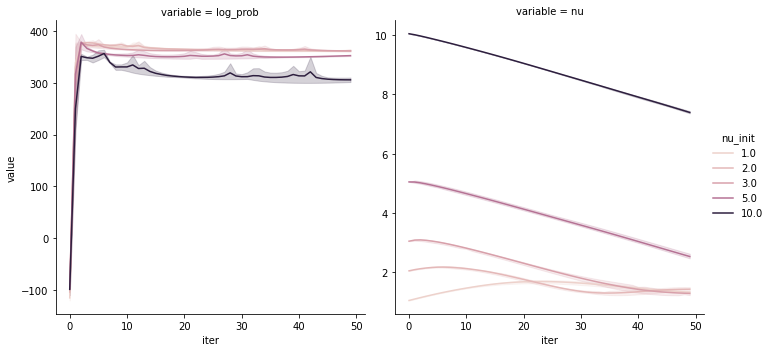
\includegraphics[width=.8\textwidth]{figures/vi-lin.png}
    \caption{Traces of the log likelihood (left) and values of the tail parameters of
    the variational approximations (true $\nu=2$). Informed initialization at $\nu=2$ leads
    to fast training and an optimal value attaining a higher log likelihood}
    \label{fig:vi-lin}
\end{figure}



\appendix

\section{External results}
The following theorem is \cite[Corollary 1]{kasahara1978tauberian}.
\begin{theorem}[Kasahara's Tauberian Theorem]
For any random variable $X$,
\[
\limsup_{x\to\infty} \frac{1}{x} \log \mathbb{P}(|X| > x^{1/\rho}) = -\alpha,
\]
if and only if
\[
\limsup_{\lambda\to\infty} \lambda^{-\frac{\rho}{\rho - 1}} \log \mathbb{E}e^{\lambda |X|} = \frac{\rho - 1}{\rho}(\alpha \rho)^{-\frac{1}{\rho - 1}}.
\]
\end{theorem}

\bibliographystyle{plain}
\bibliography{main}

\end{document}
